\subsection{Raddrizzatore di precisione}

\subsubsection{Premessa sui raddrizzatori}

I raddrizzatori sono dei circuiti il cui scopo è quello di effettuare il modulo di un segnale in ingresso preservandone la forma. In precedenti corsi di optoelettronica abbiamo incontrato alcuni semplici raddrizzatori i cui elementi circuitali chiave erano i diodi. Questi dispositivi sono in grado di portarsi in conduzione, e quindi di chiudere il ramo di circuito in cui si è posto il diodo, se la tensione al polo positivo è maggiore di quella al polo negativo; altrimenti il diodo apre il circuito. In realtà, ciò accade unicamente nel caso in cui il diodo sia ideale: per polarizzare un diodo è infatti necessario creare una differenza di tensione ai suoi capi, detta tensione di soglia $V_d$, che ha un valore di $\approx 0.6$ \si{\volt}; altrimenti il diodo risulterà come non polarizzato e dunque non in conduzione. Questo fatto, nella creazione di raddrizzatori può creare alcuni svantaggi, soprattutto se necessaria un'alta precisione (lavorando con piccoli valori di tensione): il segnale in uscita sarà con la stessa forma d'onda del segnale in entrata, ma con un offset di $-0.6$\si{\volt} dato dalla $V_d$; inoltre, se i segnali in entrata hanno valori più piccoli della tensione di soglia, il diodo non entrerà mai in conduzione. Di seguito presentiamo alcuni circuiti che risolvono in parte queste problematiche.

\subsubsection{Raddrizzatore}

\begin{wrapfigure}[16]{r}{0.5\textwidth}
  \begin{center}
    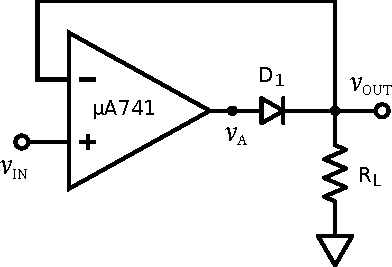
\includegraphics[width=0.350\textwidth]{../E05/latex/c_rectifier_A.pdf}
  \end{center}
  \caption{Circuito del raddrizzatore con un diodo. La resistenza di carico è $R_L=10$ \si{\kilo\ohm}.}
  \label{cir5:raddrizz_1}
\end{wrapfigure}

Analizziamo il circuito in Figura \ref{cir5:raddrizz_1}. Vogliamo dimostrare che, qualunque sia il segnale in entrata, il contributo alla tensione di uscita dato dalla tensione di soglia del diodo è trascurabile.

Innanzitutto notiamo che, dato l'alto guadagno dell'operazionale, la tensione in entrata per polarizzare il diodo è un valore molto basso (con un guadagno di $2\times 10^5$ la tensione necessaria è data da $0.6 \si{\volt}/2\times 10^5 \approx 3 \si{\micro\volt}$); dunque non dobbiamo preoccuparci che il segnale in entrata debba avere un valore minimo per far funzionare il circuito.

Vale per l'operazionale l'equazione (\ref{eq3:regola_opamp})\footnote{In realtà bisognerebbe considerare anche la dipendenza dalla frequenza. Abbiamo però notato che, ben prima che si possa apprezzare l'abbattimento dell'amplificazione, incorreremo in un altro problema dato dalla velocità di polarizzazione dei transistor all'interno dell'operazionale che ci porterà a scartare questo circuito come raddrizzatore di precisione ad alte frequenze.}
\begin{equation}
V_{A}=A (V^+-V^-)
\label{eq5:regola_opamp_NOFREQDEP}
\end{equation}
dove $V_{A}$ è la tensione all'uscita dell'amplificatore operazionale.
Valutiamo ora il circuito in due casi: $V_{in}<0$ e $V_{in}>0$\footnote{Grazie alle considerazioni sopra possiamo trascurare la tensione in ingresso necessaria per polarizzare il diodo}.

\paragraph*{Caso $V_{in}<0$}

Nel primo caso, l'OPAMP amplifica il segnale negativo in entrata sull'uscita rispettando la (\ref{eq5:regola_opamp_NOFREQDEP}) con $V_-=0$: infatti, essendo il diodo interdetto (il polo positivo è più negativo di quello negativo), non passa alcuna corrente per $R_L$ rendendo $V^-=V_{out}=0$. Inoltre, dato che l'OPAMP è in saturazione ($V^+-V^-$ diventa molto grande), $V_A \approx V_{CC}$.

\paragraph*{Caso $V_{in}>0$}

Nel secondo caso invece il diodo è in conduzione. Consideriamo dunque, come si nota dalla Figura \ref{cir5:raddrizz_1}
$$V^+=V_{in} \qquad V^-=V_{out}$$
Dato che un diodo in conduzione ha una caduta in buona approssimazione costante $V_d$, vale anche che
$$V_{A}=V_{out}+V_d$$
Sostituendo questi risultati in (\ref{eq5:regola_opamp_NOFREQDEP}) otteniamo le equazioni cercate
\begin{equation}
V_{out}=\frac{1}{1+A} (A V_{in} - V_d) \approx V_{in} \qquad V_{A} \approx V_{in}+V_d
\label{eq5:leggi_1.1}
\end{equation}

In Figura \ref{gr5:primo_raddrizzatore} presentiamo i grafici delle tensioni in funzione del tempo alla frequenza di $50$ \si{\hertz}.

\begin{figure}[ht]
 \centering
   {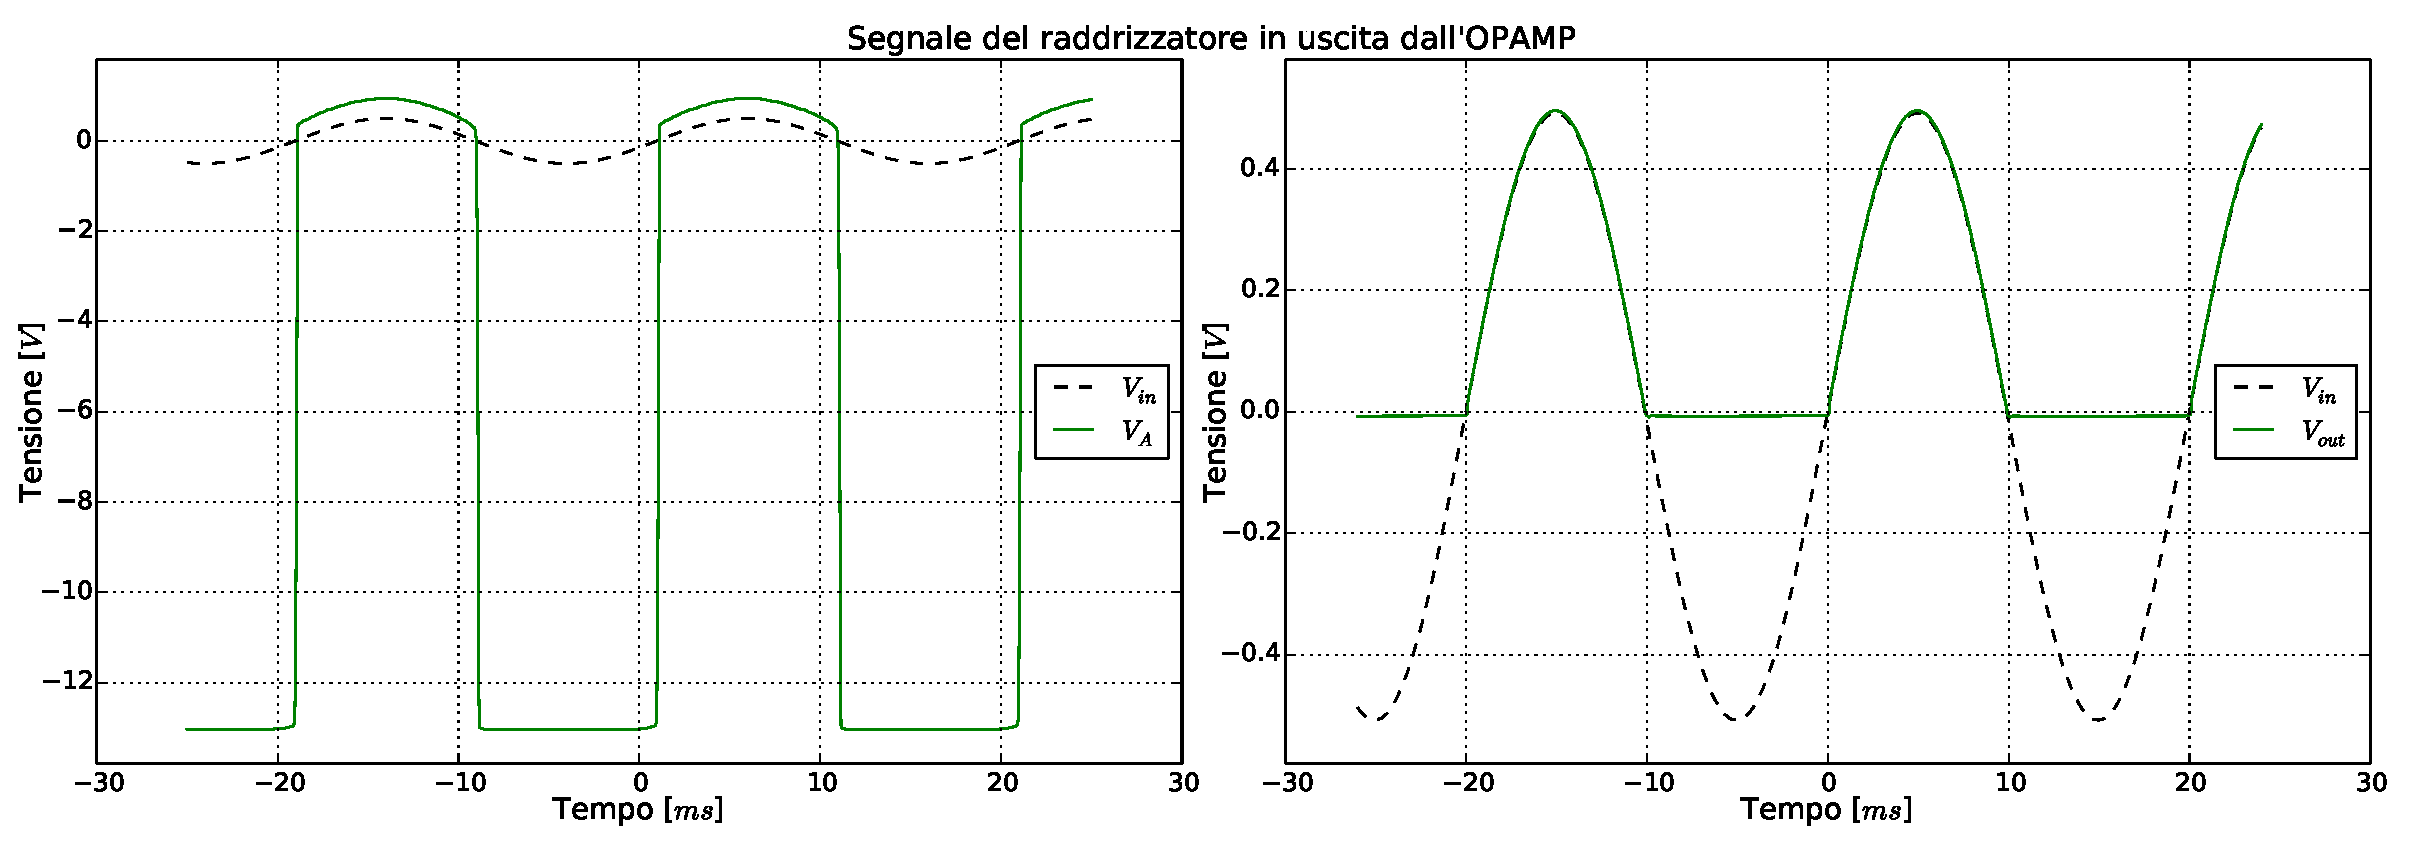
\includegraphics[width=19.5cm]{../E05/latex/unite_tempo.pdf}}
 \caption{Grafici delle tensioni in funzione del tempo. Il primo grafico è quello relativo alla tensione all'uscita del circuito $V_{out}$, il secondo alla tensione in uscita dall'OPAMP $V_A$, dove è facile vedere che l'operazionale entra in saturazione negativa.}
 \label{gr5:primo_raddrizzatore}
\end{figure}

In Figura \ref{gr5:primo_raddrizzatore_vin} presentiamo invece i grafici delle tensioni come funzioni di $V_{in}$

\begin{figure}[ht]
 \centering
   {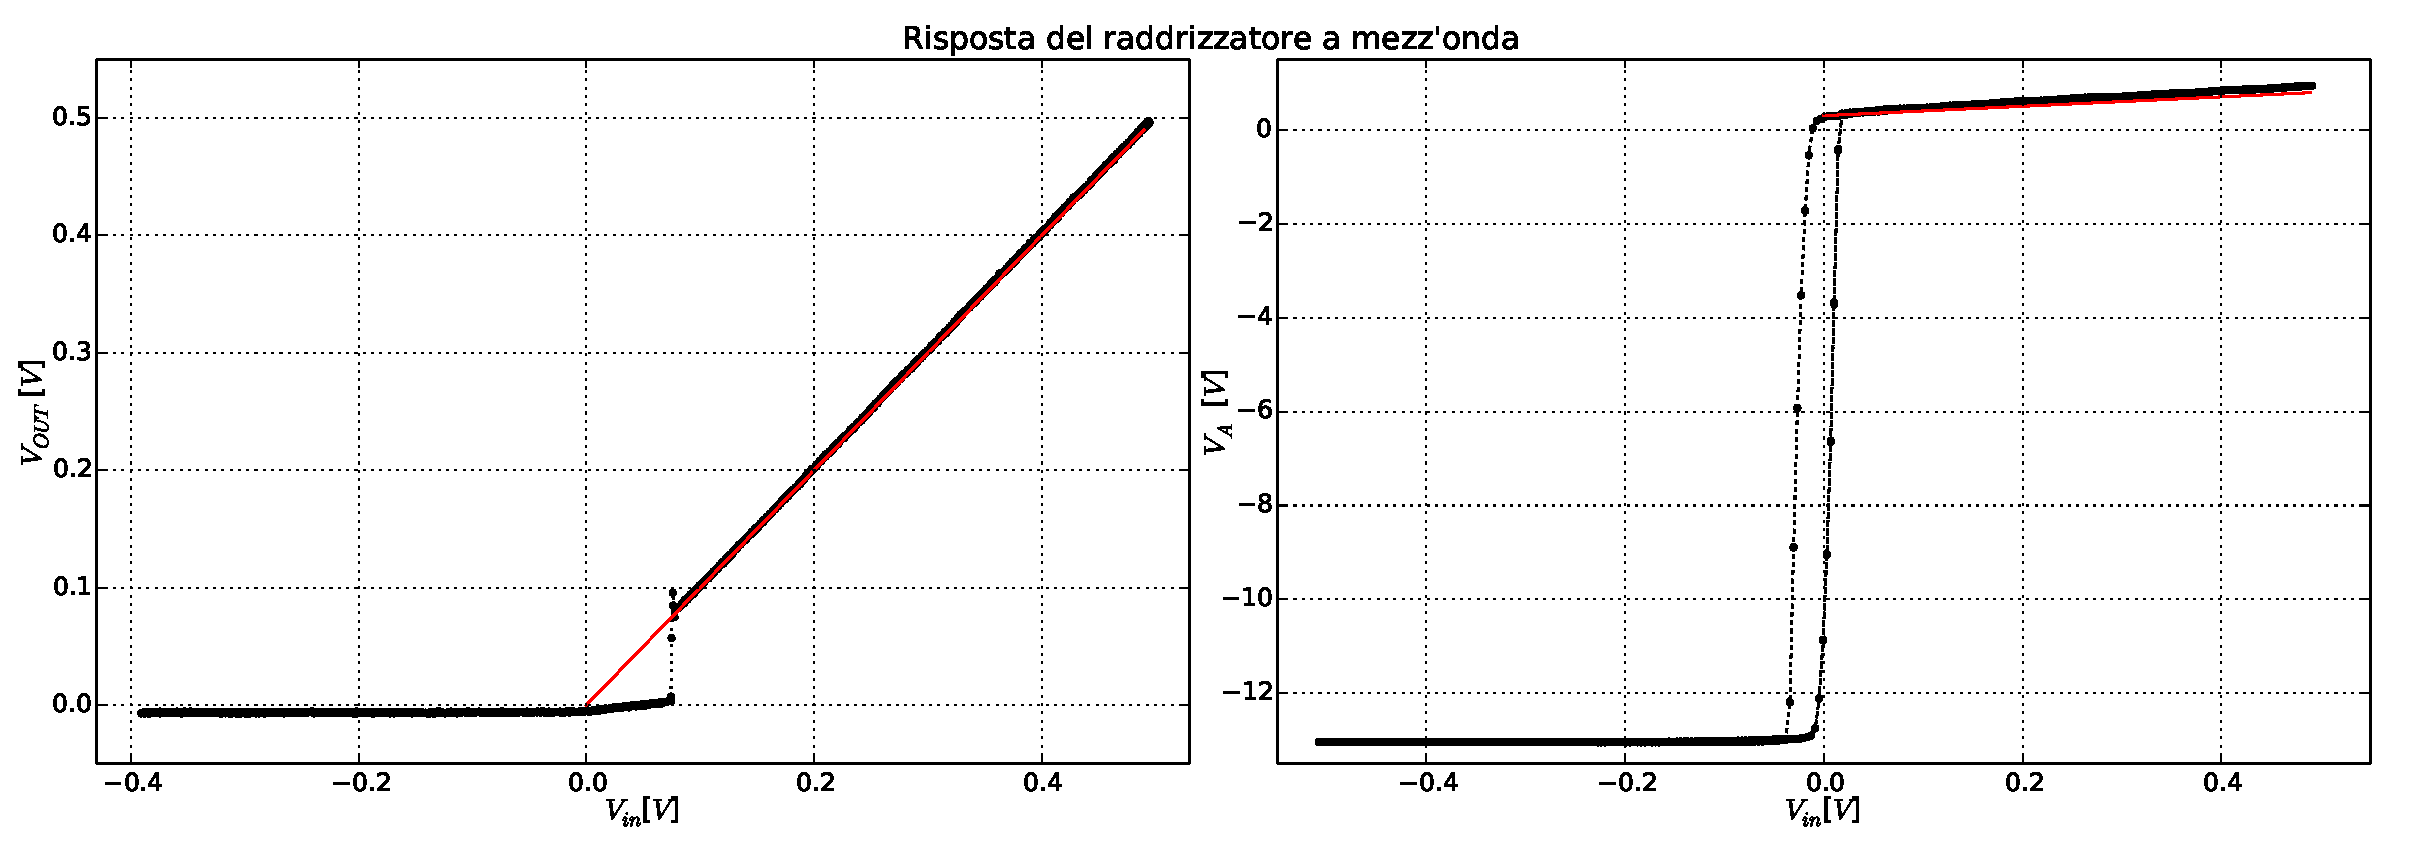
\includegraphics[width=19.5cm]{../E05/latex/u_risposta.pdf}}
 \caption{Grafici rispettivamente (da sinistra a destra) della tensione in uscita dal circuito in funzione della tensione in entrata, e della tensione in uscita dall'OPAMP in funzione della tensione in ingresso. Le leggi plottate sono per i due grafici le (\ref{eq5:leggi_1.1}).}
 \label{gr5:primo_raddrizzatore_vin}
\end{figure}

\begin{figure}[ht]
 \centering
   {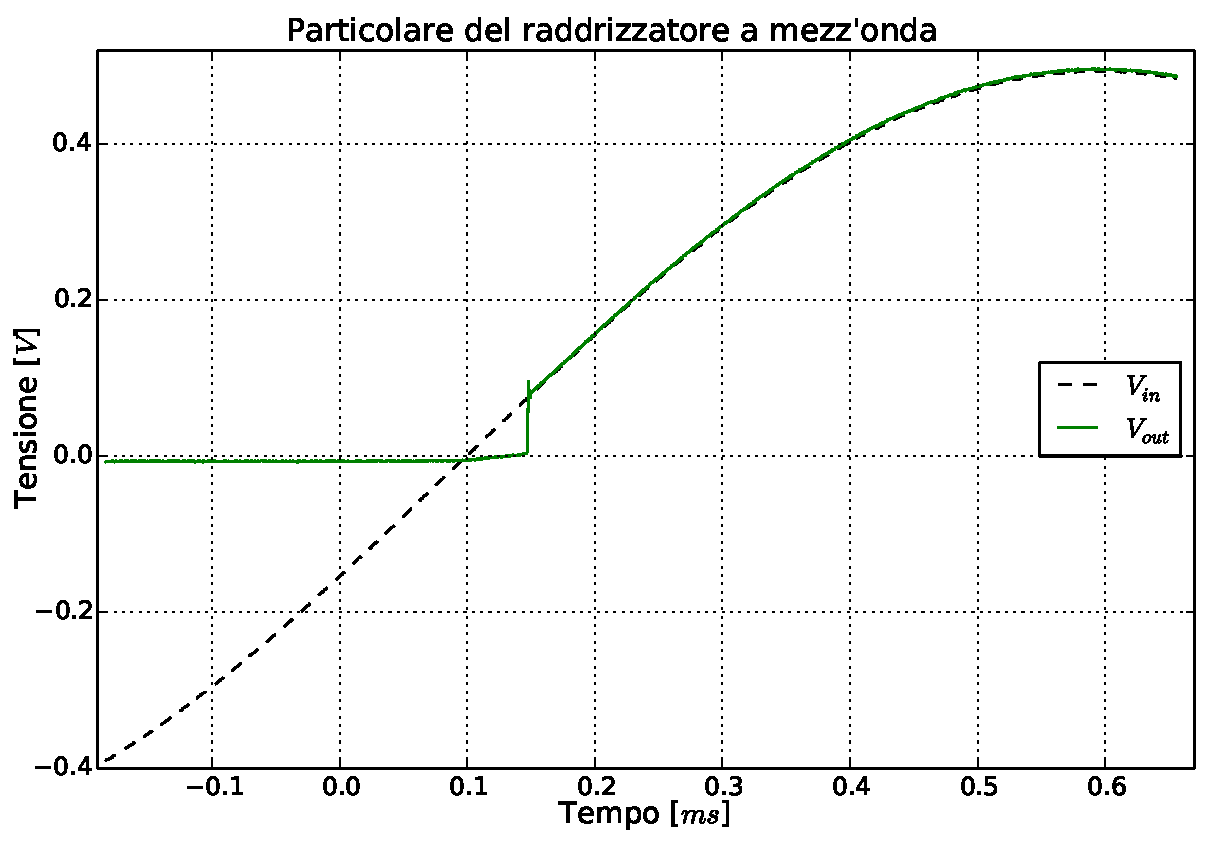
\includegraphics[width=14.5cm]{../E05/latex/zoom.pdf}}
 \caption{Grafico della tensione in entrata (tratteggiata) e della tensione in uscita dal circuito (in verde) in funzione del tempo. Si nota il fenomeno esposto nel paragrafo.}
 \label{gr5:problema}
\end{figure}

Dal plot del segnale in entrata ed in uscita in funzione del tempo alla frequenza di 2 \si{\kilo\hertz} (grafico in Figura \ref{gr5:problema}), possiamo notare un troncamento della forma d'onda del segnale in uscita. Abbiamo ipotizzato che tale fenomeno fosse dovuto alla limitata velocità che i transistor all'interno dell'operazionale hanno di passare dalla saturazione all'interdizione; tale fenomeno è anche amplificato dal fatto che, quando il diodo è interdetto, $V_{A} \approx -V_{CC}$: il segnale deve quindi passare da una tensione di saturazione negativa alla tensione necessaria per raddrizzare il segnale in uscita in un tempo troppo breve, e ad alte frequenze ciò risulta in un troncamento. Per risolvere tale problema utilizziamo il circuito esposto al sottoparagrafo successivo.

\subsubsection{Raddrizzatore ottimizzato}

\begin{wrapfigure}[16]{l}{0.5\textwidth}
  \begin{center}
    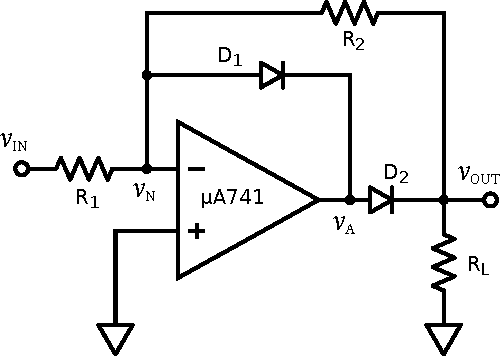
\includegraphics[width=0.350\textwidth]{../E05/latex/c_rectifier_B.pdf}
  \end{center}
  \caption{Circuito del raddrizzatore a semionda ottimizzato. La resistenza di carico è $R_L=10$ \si{\kilo\ohm}, mentre $R_1=R_2=10$ \si{\kilo\ohm}.}
  \label{cir5:raddrizz_2}
\end{wrapfigure}

Per risolvere il problema visto in precedenza, utilizziamo un secondo diodo posto come nel in Figura \ref{cir5:raddrizz_2} e un circuito di retroazione controllata in guadagno. Anche in questo caso dobbiamo valutare la risposta del circuito in casi diversi: $V_{in}=0$, $V_{in}>0$ e $V_{in}<0$.

\paragraph*{Caso $V_{in}=0$}

Nel primo caso abbiamo entrambi i diodi interdetti. Infatti, se la tensione in ingresso è nulla non vi è la tensione necessaria a polarizzare i diodi, che rimangono non polarizzati. Dunque $V_{out}=V_{A}=0$.

\paragraph*{Caso $V_{in}>0$}

Tenendo conto della (\ref{eq5:regola_opamp_NOFREQDEP}), considerando che $V_{in}$ viene portata sull'ingresso invertente, la tensione su $V_{A}$ sarà negativa e quindi più bassa di $V_{out}$: dunque $D_2$ sarà interdetto. Allo stesso tempo il polo positivo di $D_1$ è più positivo (a comune virtuale) di quello negativo ($V_{A}$), dunque tale diodo risulta in conduzione. Inoltre, $V_{out}$ risulta nulla in quanto sul ramo di circuito identificato da $R_2$ e $R_L$ non passa corrente (sono collegate rispettivamente a comune virtuale e comune). $V_{A}$ sarà invece fissata dalla tensione di soglia del diodo, cioè $V_{A}=-V_d$.

\paragraph*{Caso $V_{in}<0$}

Con considerazioni analoghe al caso precedente, possiamo concludere che $D_1$ risulta interdetto, mentre $D_2$ in conduzione. Quindi il circuito è un amplificatore invertente di segnale con guadagno $-R_2/R_1$.

Valutiamo il contributo del diodo nella tensione di uscita del circuito $V_{out}$ e dell'operazionale $V_{A}$. Consideriamo le correnti nel nodo $V_N$
$$\frac{V_{in}-V_N}{R_1} + \frac{V_{out}-V_N}{R_2} = 0$$
Osservando che $V_N$ è a ground virtuale, che $V_{out}=V_{A}-V_d$, e considerando l'operazionale come ideale e che vale che $V_{out}=V_{A}-V_d$, dalla (\ref{eq5:regola_opamp_NOFREQDEP}) otteniamo
\begin{equation}
V_{out}=-\frac{R_2}{R_1}V_{in} \qquad V_A = \frac{R_2}{R_1} V_{in} + V_d
\label{eq5:v_out_ottimizzato}
\end{equation}

In Figura \ref{gr5:secondo_raddrizzatore} presentiamo il grafico della tensione.

\begin{figure}[ht]
 \centering
   {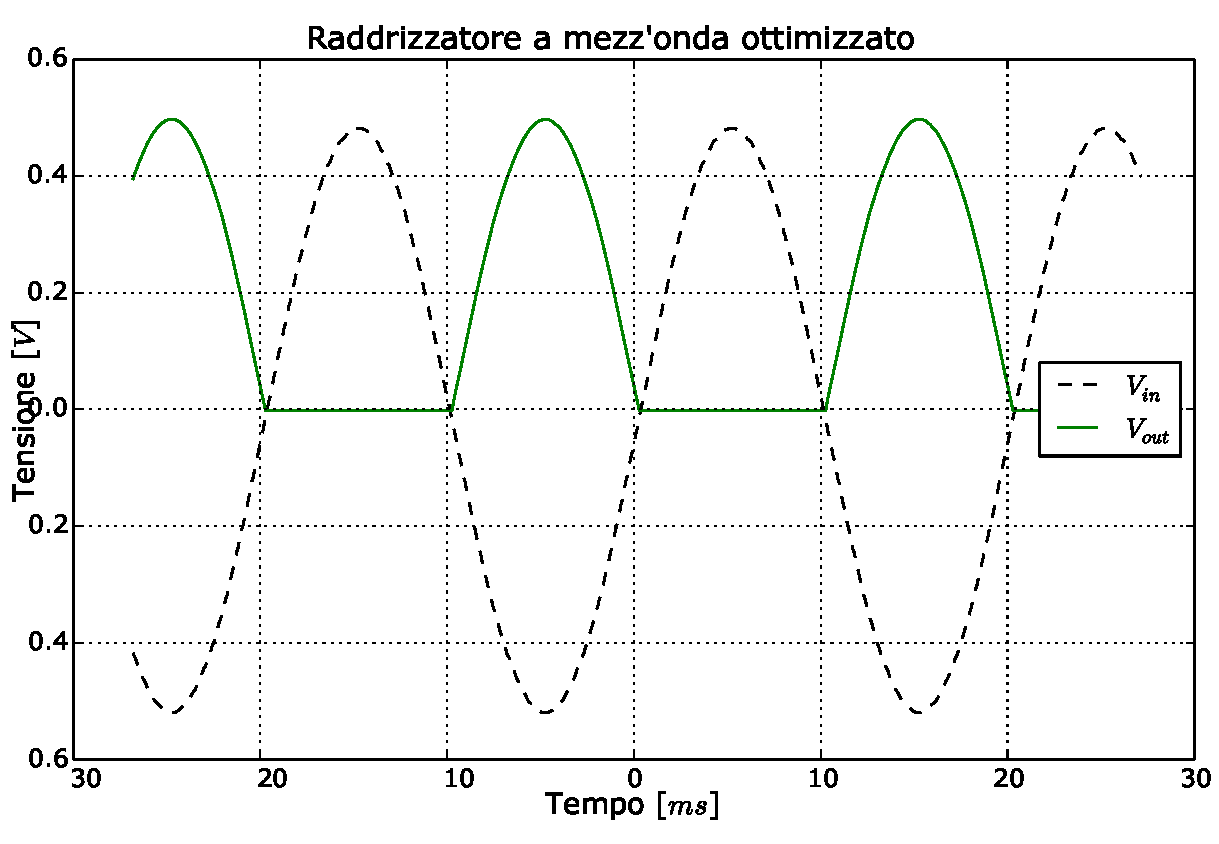
\includegraphics[width=14.5cm]{../E05/latex/radd_ott.pdf}}
 \caption{Grafico delle tensioni in funzione del tempo. Notiamo che il guadagno negativo quando $V_{in}<0$, plausibile con (\ref{eq5:v_out_ottimizzato}).}
 \label{gr5:secondo_raddrizzatore}
\end{figure}